%
%
%% Based on the style files for ACL 2018, NAACL 2018/19, which were
%% Based on the style files for ACL-2015, with some improvements
%%  taken from the NAACL-2016 style
%% Based on the style files for ACL-2014, which were, in turn,
%% based on ACL-2013, ACL-2012, ACL-2011, ACL-2010, ACL-IJCNLP-2009,
%% EACL-2009, IJCNLP-2008...
%% Based on the style files for EACL 2006 by 
%%e.agirre@ehu.es or Sergi.Balari@uab.es
%% and that of ACL 08 by Joakim Nivre and Noah Smith

\documentclass[11pt,a4paper]{article}
\usepackage[hyperref]{acl2019}
\aclfinalcopy % Uncomment this line for the final submission
%\def\aclpaperid{***} %  Enter the acl Paper ID here


\usepackage{times}
\usepackage{url}
\usepackage{latexsym}
%\usepackage{fixltx2e}
\usepackage{fixmath}
\usepackage{etex}

\usepackage[utf8]{inputenc}
\usepackage{fontenc}
\DeclareUnicodeCharacter{1A1}{o}
\DeclareUnicodeCharacter{1B0}{u}
\let\vec=\mathbold

\usepackage[english]{babel}
\usepackage{booktabs}
\usepackage{amsmath}
\usepackage{enumitem}
\usepackage[amsmath,standard,thmmarks]{ntheorem}
\usepackage{tabularx}
\usepackage{tikz}
\usepackage{float}
\usepackage{subcaption}
\usetikzlibrary{calc}
\usetikzlibrary{chains}
\usetikzlibrary{patterns}
\usetikzlibrary{shapes}

\usepackage{enumitem}
\usepackage{multirow}
\usepackage{adjustbox}



\theoremnumbering{arabic}
\theoremstyle{plain}
\RequirePackage{latexsym}
\theoremsymbol{\ensuremath{_\Box}}
\theorembodyfont{\itshape}
\theoremheaderfont{\normalfont\bfseries}
\theoremseparator{}
\newtheorem{fact}{Fact}

\newcommand{\figref}[1]{\figurename~\ref{#1}}
%\addto\captionsenglish{\renewcommand{\figurename}{Fig.}}
\newcommand*{\arcij}{i \rightarrow j}

\makeatletter
\def\Let@{\def\\{\notag\math@cr}}
\makeatother

\newcommand*{\MLP}{MLP}
\newcommand*{\CCG}{CCG}
\newcommand*{\CCD}{CCD}
\newcommand*{\DM}{DM}
\newcommand*{\LF}{LF}
\newcommand*{\LP}{LP}
\newcommand*{\LR}{LR}
%\newcommand*{\LR}{\mathit{LR}}
\newcommand*{\LM}{LM}
\newcommand*{\PAS}{PAS}
\newcommand*{\PCEDT}{PCEDT}
\newcommand*{\PSD}{PSD}
\newcommand*{\SDP}{SDP}
\newcommand*{\SET}[1]{\{#1\}}
\newcommand*{\UF}{UF}
\newcommand*{\UP}{UP}
\newcommand*{\UR}{UR}
\DeclareMathOperator*{\argmax}{arg\,max}
\DeclareMathOperator*{\argmin}{arg\,min}
%\DeclareMathOperator*{\max}{max}
%\DeclareMathOperator*{\min}{min}

\def\fscore{F$_1$}

\usepackage{microtype}
\usepackage{multicol}

\makeatletter
\useshorthands{"}%
\defineshorthand{"-}{\nobreak-\bbl@allowhyphens}%
\defineshorthand{"=}{\nobreak--\bbl@allowhyphens}%
\makeatother

\newcommand\BibTeX{B\textsc{ib}\TeX}

%\title{End-to-End Negation Resolution with Bilinear Attention}
\title{End"-to"-End Negation Resolution as Graph Parsing}

\author{
    Robin Kurtz$^\spadesuit$, Stephan Oepen$^\clubsuit$, Marco Kuhlmann$^\spadesuit$ \\ % name
    {\normalsize $\spadesuit$ Linköping University, Department of Computer and Information Science}\\ % basic academic or research unit
    {\normalsize $\clubsuit$ University of Oslo, Department of Informatics}\\ % basic academic or research unit
 \texttt{robin.kurtz@liu.se}, \texttt{oe@ifi.uio.no}, \texttt{marco.kuhlmann@liu.se}
 }   % email


\date{}

\begin{document}
\maketitle
\begin{abstract}
  We present a neural end-to-end architecture for negation resolution
  based on a formulation of the task as a graph parsing problem.
  Our approach allows for the straightforward inclusion of many types
  of graph-structured features without the need for
  representation-specific heuristics.
  In our experiments, we specifically gauge the usefulness of
  syntactic information for negation resolution.
  Despite the conceptual simplicity of our architecture, we achieve
  state-of-the-art results on the Conan Doyle benchmark dataset,
  including a new top result for our best model.
\end{abstract}

\section{Introduction}
\label{sec:introduction}

Negation resolution (NR), the task of detecting negation and determining its scope,
is relevant for a large number of applications in
natural language processing, and has been the subject of several
contrastive research efforts
\citep{Mor:Bla:12,Oep:Ovr:Bjo:17,Far:Oep:Ovr:18}.
In this paper we cast NR as a graph parsing problem.
More specifically, we represent negation \emph{cues} and corresponding \emph{scopes} as a
bi-lexical graph and learn to predict this graph from the tokens.
Under this representation, we may apply any dependency graph
parser to the task of negation resolution.
The specific parsing architecture that we use in this paper extends that of \citet{dozat2018simpler}.


\paragraph{Contributions}
This work
(a)~rationally reconstructs the previous state of the art in negation
resolution;
(b)~develops a novel approach to the problem based on general graph
parsing techniques;
(c)~proposes and evaluates different ways of integrating `external'
grammatical information;
(d)~gauges the utility of morpho-syntactic pre-processing at different
levels of accuracy;
(e) shifts experimental focus (back) to a complete, end-to-end
perspective on the task; and 
(f)~reflects on uncertainty in judging experimental findings,
including thorough significance testing.

%\begin{trivlist}
%\item\relax \emph{Paper Structure.}
\paragraph{Paper Structure}
In the following Section~\ref{sec:related}, we review selected related work
on negation resolution.
Section~\ref{sec:background} describes the specific NR task that we address in this paper.
In Section~\ref{sec:model} we present our new encoding of negations and our
parsing model, followed by the description of our experiments and results in
Section~\ref{sec:experiments}.
We discuss these results in Section~\ref{sec:discussion} and summarize our findings in
Section~\ref{sec:conclusion}.

%\end{trivlist}
%\begin{itemize}
%    \item 2012 *SEM
%    \item only dataset to have events, scopes and cues for negation
%    \item 2017 and 2018 EPE
%    \item Sherlock and bug
%    \item general method with NNs, can scale
%    \item \dots
%    \item 
%        \cite{oepen20172017,fares20182018}
%        \cite{lapponi2012uio,lapponi2017epe}
%\end{itemize}

\section{Related Work}
\label{sec:related}

%\begin{itemize}
%    \item 2012 *SEM
%    \item Sherlock, UiO1, 2014 MRS Crawler, Fancellu 2016\&2018, Sergeeva 2019
%    \item negation datasets
%    \item \dots
%    \item \cite{morante2012sem,morante2012conandoyleneg}
%        \cite{lapponi2012uio}
%        \cite{read2012uio1}
%        \cite{packard2014simple}
%        \cite{fancellu2016neural}
%        \cite{sergeeva2019neural}
%        \cite{szarvas2008bioscope,jimenez-zafra0corpora,liu2018negpar}
%        \cite{elming2013downstream}
%\end{itemize}

While there exist a variety of datasets that annotate negation
\citep{jimenez-zafra0corpora}, the BioScope
\citep{szarvas2008bioscope} and Conan Doyle datasets
\citep[ConanDoyle-neg; ][]{morante2012conandoyleneg} are most commonly used for evaluation.
The latter was created for the shared task at *SEM~2012
\citep{Mor:Bla:12}, where competing systems needed to predict both
negation \emph{cues} (linguistic expressions of negation) and their
corresponding \emph{scopes}, i.e.\ the part of the utterance being
negated.
Cues can be simple negation markers (such as \textit{not} or \textit{without}), but may also
consist of multiple words (i.e.\ \textit{neither~\dots~nor}), or be
mere affixes (i.e.\ \textit{in}frequent or clue\textit{less}).
In contrast to other datasets, ConanDoyle-neg also annotates
negated \emph{events} that are part of the scopes.

\begin{figure*}
  \centering
  \includegraphics[width=.9\textwidth, trim=0 0 0 210, clip=true]{sharp3.pdf}
  \caption{An example of how overlapping ConanDoyle-neg annotations are
  converted to flat sequences of labels in \textsc{Sherlock}.
  In this example, an in-scope token is labelled with \texttt{N}, a cue
  with \texttt{CUE}, a negated event with \texttt{E}, a negation stop
  with \texttt{S}, and an out-of-scope token with \texttt{O}. Illustration taken from \citet{Lap:Oep:Ovr:17}.}
\label{fg:sherlock}
\end{figure*}

The analysis of negation is divided into two related sub"-tasks,
\emph{cue detection} and \emph{scope resolution}.
While cue detection is mostly dependent on lexical or morphological
features, relating cues to scopes is a structured prediction problem and will likely benefit from an analysis of
morpho"-syntactic or surface"-semantic properties.
The UiO$_2$ system \textsc{Sherlock} \citep{Lap:Vel:Ovr:12}, the winner
of the open track of the *SEM~2012 shared task, uses morpho-syntactic parts of speech and syntactic dependencies
to classify tokens as either in"-scope or out"-of"-scope using a conditional
random field~(CRF).
Another CRF further classifies scope tokens as events, and a heuristic
is applied to distribute scope tokens to their respective cues.
The \textsc{Sherlock} system was subsequently used by \citet{elming2013downstream} to
evaluate various dependency conversions, and
similarly served as one of three reference `downstream' applications in the 2017 Extrinsic Parser Evaluation initiative
(EPE; \citealp{Oep:Ovr:Bjo:17}).
The best results from this evaluation define the state of the art in NR.

Deviating from the original *SEM~2012 setup, \citet{Pac:Ben:Rea:14} simplified
the task to only evaluate the performance on finding scope
tokens, assuming gold-standard information about negation cues.
\citet{fancellu2016neural,fancellu2018neural} continued this trend, additionally
treating each negation instance separately, and successfully used BiLSTM
(bidirectional Long Short"-Term Memory recurrent neural networks;
\citealp{hochreiter1997long}).
Recently, \citet{sergeeva2019neural} used pre"-trained transformers
\citep{vaswani2017attention}, namely BERT \citep{devlin2019bert}, to
further improve performance, albeit on a derivative of the original
dataset \citep{liu2018negpar}.
Using BERT in a two"-stage sequence"-labelling approach on the original
ConanDoyle-neg corpus and other relevant negation corpora,
\citet{khandelwal2020negbert} successfully improved previous results by a
considerable margin.
The 2018 follow-up to the EPE shared task \citep{Far:Oep:Ovr:18} again used \textsc{Sherlock}
to evaluate parsing performance, this time restricting itself to participating systems in the
co"-located 2018 CoNLL Shared Task on Universal Dependency
Parsing~\citep{zeman2018conll}.


\section{Task and Data}
\label{sec:background}

We target the original *SEM 2012 shared task and aim to predict both negation cues and their scopes.
We compare our approach with the baseline \textsc{Sherlock} system and the state-of-the-art systems identified through the EPE shared tasks.

%\begin{figure*}
%  \centering
%  %\resizebox{\textwidth}{!}{
%  %\small
%  \begin{tikzpicture}[start chain, node distance=-0.3em, cra/.style={out=-90, ->, in=-90}, arc/.style={out=90, ->, in=90}, arc label/.style={font=\small, inner sep=1pt, fill=white}, execute at begin node=\strut]
%    %\node[on chain, name=t0] {Mr.};
%    %\node[on chain, name=t1] {Sherlock};
%    %\node[on chain, name=t2] {Holmes,};
%    %\node[on chain, name=t1] {ROOT};
%    %\node[on chain, name=t2] {\dots};
%    %\node[on chain, name=t3] {who};
%    %\node[on chain, name=t4] {was};
%    %\node[on chain, name=t5] {usually};
%    %\node[on chain, name=t6] {very};
%    %\node[on chain, name=t7] {late};
%    %\node[on chain, name=t8] {in};
%    %\node[on chain, name=t9] {the};
%    %\node[on chain, name=t10] {mornings,};
%    %\node[on chain, name=t11] {save};
%    %\node[on chain, name=t12] {upon};
%    \node[on chain, name=t13] {those};
%    \node[on chain, name=t14] {not};
%    \node[on chain, name=t15] {infrequent};
%    \node[on chain, name=t16] {occasions};
%    \node[on chain, name=t17] {when};
%    \node[on chain, name=t18] {he};
%    \node[on chain, name=t19] {was};
%    \node[on chain, name=t20] {up};
%    \node[on chain, name=t21] {all};
%    \node[on chain, name=t22] {night,};
%    \node[on chain, name=t23] {\dots};
%    %\node[on chain, name=t23] {was};
%    %\node[on chain, name=t24] {seated};
%    %\node[on chain, name=t25] {at};
%    %\node[on chain, name=t26] {the};
%    %\node[on chain, name=t27] {breakfast};
%    %\node[on chain, name=t28] {table.};
%
%    %\draw[thick] ($(t11.north) + (0.00, 0)$) edge[arc]   ($(t3.north) - (0.00, 0)$);
%    %\draw[] ($(t11.north) + (0.00, 0)$) edge[arc]   ($(t4.north) - (0.00, 0)$);
%    %\draw[] ($(t11.north) + (0.00, 0)$) edge[arc]   ($(t5.north) - (0.00, 0)$);
%    %\draw[thick] ($(t11.north) + (0.00, 0)$) edge[arc]   ($(t6.north) - (0.00, 0)$);
%    %\draw[] ($(t11.north) + (0.00, 0)$) edge[arc]   ($(t7.north) - (0.00, 0)$);
%    %\draw[] ($(t11.north) + (0.00, 0)$) edge[arc]   ($(t8.north) - (0.00, 0)$);
%    %\draw[] ($(t11.north) + (0.00, 0)$) edge[arc]   ($(t9.north) - (0.00, 0)$);
%    %\draw[] ($(t11.north) + (0.00, 0)$) edge[arc]   ($(t10.north) - (0.00, 0)$);
%    %\draw[] ($(t11.north) + (0.00, 0)$) edge[arc]   ($(t11.north) - (0.00, 0)$);
%    %\draw[] ($(t11.north) + (0.00, 0)$) edge[arc]   ($(t12.north) - (0.00, 0)$);
%    %\draw[] ($(t11.north) + (0.00, 0)$) edge[arc]   ($(t13.north) - (0.00, 0)$);
%    %\draw[] ($(t11.north) + (0.00, 0)$) edge[arc]   ($(t15.north) - (0.00, 0)$);
%    %\draw[] ($(t11.north) + (0.00, 0)$) edge[arc]   ($(t16.north) - (0.00, 0)$);
%    %\draw[] ($(t11.north) + (0.00, 0)$) edge[arc]   ($(t17.north) - (0.00, 0)$);
%    %\draw[] ($(t11.north) + (0.00, 0)$) edge[arc]   ($(t18.north) - (0.00, 0)$);
%    %\draw[] ($(t11.north) + (0.00, 0)$) edge[arc]   ($(t19.north) - (0.00, 0)$);
%    %\draw[] ($(t11.north) + (0.00, 0)$) edge[arc]   ($(t20.north) - (0.00, 0)$);
%    %\draw[] ($(t11.north) + (0.00, 0)$) edge[arc]   ($(t21.north) - (0.00, 0)$);
%    %\draw[] ($(t11.north) + (0.00, 0)$) edge[arc]   ($(t22.north) - (0.00, 0)$);
%    
%    \draw[] ($(t14.south) + (0.00, 0)$) edge[cra]   ($(t13.south) - (0.00, 0)$);
%    \draw[thick] ($(t14.south) + (0.00, 0)$) edge[cra]   ($(t15.south) - (0.00, 0)$);
%    \draw[] ($(t14.south) + (0.00, 0)$) edge[cra]   ($(t16.south) - (0.00, 0)$);
%    \draw[] ($(t14.south) + (0.00, 0)$) edge[cra]   ($(t17.south) - (0.00, 0)$);
%    \draw[] ($(t14.south) + (0.00, 0)$) edge[cra]   ($(t18.south) - (0.00, 0)$);
%    \draw[] ($(t14.south) + (0.00, 0)$) edge[cra]   ($(t19.south) - (0.00, 0)$);
%    \draw[] ($(t14.south) + (0.00, 0)$) edge[cra]   ($(t20.south) - (0.00, 0)$);
%    \draw[] ($(t14.south) + (0.00, 0)$) edge[cra]   ($(t21.south) - (0.00, 0)$);
%    \draw[] ($(t14.south) + (0.00, 0)$) edge[cra]   ($(t22.south) - (0.00, 0)$);
%
%    \draw[red] ($(t15.south) + (0.00, 0)$) edge[cra]   ($(t13.south) + (0.09, 0)$);
%    \draw[red,thick] ($(t15.south) + (0.00, 0)$) edge[cra]   ($(t15.south) + (0.09, 0)$);
%    \draw[red] ($(t15.south) + (0.00, 0)$) edge[cra]   ($(t16.south) + (0.09, 0)$);
%    \draw[red] ($(t15.south) + (0.00, 0)$) edge[cra]   ($(t17.south) + (0.09, 0)$);
%    \draw[red] ($(t15.south) + (0.00, 0)$) edge[cra]   ($(t18.south) + (0.09, 0)$);
%    \draw[red] ($(t15.south) + (0.00, 0)$) edge[cra]   ($(t19.south) + (0.09, 0)$);
%    \draw[red] ($(t15.south) + (0.00, 0)$) edge[cra]   ($(t20.south) + (0.09, 0)$);
%    \draw[red] ($(t15.south) + (0.00, 0)$) edge[cra]   ($(t21.south) + (0.09, 0)$);
%    \draw[red] ($(t15.south) + (0.00, 0)$) edge[cra]   ($(t22.south) + (0.09, 0)$);
%
%    \draw[] ($(t15.north) + (0.09, 0)$) edge[arc]   ($(t15.north) - (0.00, 0)$);
%
%    %\node[name=r0, above of=t11, yshift=3cm] {\small cue};
%    %\draw[] (r0) edge[style={->}] (t11.north);
%    \node[name=r1, above of=t14, yshift=3cm] {\small cue};
%    \draw[] (r1) edge[style={->}] (t14.north);
%    \node[name=r2, above of=t15, yshift=3cm] {\small cue};
%    \draw[] (r2) edge[style={->}] (t15.north);
%
%  \end{tikzpicture}
%  %}
%  \caption{A sample sentence}
%  \label{fig:neg_graph}
%\end{figure*}

\begin{figure*}
  \centering
  %\resizebox{\textwidth}{!}{
  %\small
  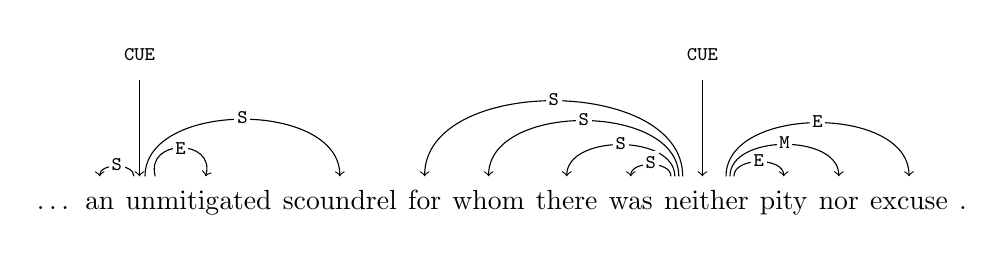
\begin{tikzpicture}[start chain, node distance=-0.3em, cra/.style={out=-90, ->, in=-90}, arc/.style={out=90, ->, in=90}, arc label/.style={font=\scriptsize, inner sep=1pt, fill=white}, execute at begin node=\strut]

    %\node[on chain, name=t5] {The};
    %\node[on chain, name=t6] {man};
    %\node[on chain, name=t7] {was};
    %\node[on chain, name=t8] {a};
    %\node[on chain, name=t9] {danger};
    %\node[on chain, name=t10] {to};
    %\node[on chain, name=t11] {the};
    %\node[on chain, name=t12] {community,};
    %\node[on chain, name=t121] {,};
    \node[on chain, name=t121] {\dots};
    \node[on chain, name=t13] {an};
    \node[on chain, name=t14] {unmitigated};
    \node[on chain, name=t15] {scoundrel};
    \node[on chain, name=t16] {for};
    \node[on chain, name=t17] {whom};
    \node[on chain, name=t18] {there};
    \node[on chain, name=t19] {was};
    \node[on chain, name=t20] {neither};
    \node[on chain, name=t21] {pity};
    \node[on chain, name=t22] {nor};
    \node[on chain, name=t23] {excuse};
    \node[on chain, name=t231] {.};

    %\path ($(t20.north) - (0.10, 0)$) edge [out=90,in=90,looseness=8] node[above] {} ($(t20.north) + (0.20, 0)$);
    \draw[] ($(t14.north) - (0.82, 0)$) edge[arc]  node[arc label]{\texttt{S}} ($(t13.north) - (0.00, 0)$);
    \draw[] ($(t14.north) - (0.68, 0)$) edge[arc] node[arc label]{\texttt{S}}  ($(t15.north) - (0.00, 0)$);
    \draw[] ($(t14.north) - (0.55, 0)$) edge[loop above, looseness=2, ->] node[arc label, below=-1ex]{\texttt{E}} ($(t14.north) + (0.09, 0)$);

    \draw[] ($(t20.north) - (0.30, 0)$) edge[arc] node[arc label]{\texttt{S}}  ($(t16.north) - (0.00, 0)$);
    \draw[] ($(t20.north) - (0.35, 0)$) edge[arc] node[arc label]{\texttt{S}}  ($(t17.north) - (0.00, 0)$);
    \draw[] ($(t20.north) - (0.40, 0)$) edge[arc] node[arc label]{\texttt{S}} ($(t18.north) - (0.00, 0)$);
    \draw[] ($(t20.north) - (0.45, 0)$) edge[arc]  node[arc label]{\texttt{S}} ($(t19.north) - (0.00, 0)$);
    %\draw[] ($(t20.north) - (0.10, 0)$) edge[loop above, looseness=8, ->] node[arc label]{mwc}  ($(t20.north) + (0.15, 0)$);
    \draw[] ($(t20.north) + (0.35, 0)$) edge[arc]  node[arc label]{\texttt{E}} ($(t21.north) + (0.00, 0)$);
    \draw[] ($(t20.north) + (0.30, 0)$) edge[arc]  node[arc label]{\texttt{M}} ($(t22.north) - (0.00, 0)$);
    \draw[] ($(t20.north) + (0.25, 0)$) edge[arc]  node[arc label]{\texttt{E}} ($(t23.north) - (0.00, 0)$);

    \node[name=r1, above of=t14, yshift=2cm, xshift=-0.75cm] {\scriptsize \texttt{CUE}};
    \draw[] (r1) edge[style={->}] ($(t14.north) - (0.75, 0)$) ;

    \node[name=r2, above of=t20, yshift=2cm, xshift=-0.05cm] {\scriptsize \texttt{CUE}};
    \draw[] (r2) edge[style={->}] ($(t20.north) - (0.05, 0)$);

  \end{tikzpicture}
  %}
  \caption{An example of how ConanDoyle-neg annotations are converted to a
      dependency"-style graph structure.
  We omit the special root node $r_0$ and mark roots instead with vertical
  arcs.
  The arcs are labelled for {scope} (\texttt{S}), {event}
  (\texttt{E}), and {multi"-word"-cue} (\texttt{M}).
  }
  \label{fig:neg_graph}
\end{figure*}
%\begin{itemize}
%    \item how are negations encoded
%    \item detect cues vs.~gold cues
%    \item sherlock system
%    \item kiperwasser, dozat parsing
%    \item \cite{kiperwasser2016simple,dozat2018simpler}
%    \item dot product attention aus everything is attention
%    \item \cite{vaswani2017attention}
%    \item gcn von kipf\&welling 2017 und marcheggiani 2017 aber auch fancellu 2018
%    \item \cite{kipf2017semisupervised,marcheggiani2017encoding}
%    \item \dots
%\end{itemize}

\subsection{Data}

The negation data of *SEM 2012 consists of selected Sherlock Holmes stories from the works of Arthur
Conan Doyle, and contains 3,644 sentences in the training set, 787
sentences in the development set, and 1,089 sentences in the evaluation
set.
The corpus annotates a total of 1,420 instances of negation.
Several sentences contain two or more instances of negation, while 4,294 sentences do not contain any at all.

Negation instances are annotated as tri-partite structures:
Negation \emph{cues} can be full tokens, multi"-word expressions, or
affixal sub-tokens.
For each cue, its \emph{scope} is defined as the possibly discontinuous
sequence of (sub-)tokens affected by the negation.
Additionally, a subset of in-scope tokens can be marked as
negated \emph{events} (or \emph{states}), provided that the sentence
is factual and the events in question did not take place. 
For sentences containing multiple negation instances, their respective
scope and event spans may nest or overlap.

\iffalse
The annotations contain linguistic signals of negations, \emph{cues},
that can be either simple single token cues, multi"-word cues or
affixal cues.
Each cue is assigned a \emph{scope}, that is tokens that are affected
by the negation, and negated \emph{events}, scope tokens that are the
focus of the negation and are factual.
As there may be multiple negation instances in one sentence, and
scopes may overlap or nest within each other.
\fi

%\begin{figure}[]
%    \centering
%    \caption{Nice figure showing negation}
%    \label{fig:negation}
%\end{figure}

The systems submitted to the EPE~2017 and 2018 tasks work on
`raw', unsegmented text, and apply different segmentation strategies.
To evaluate these systems in the context of negation resolution, 
the gold"-standard negation annotations have to
be retrofitted to each system's output.
Each system is then tested against their own
`personalized' gold standard.
For more information on this projection procedure, we refer
to \citet{Lap:Oep:Ovr:17}.

\subsection{Baseline System}

As in the EPE shared tasks, our baseline is the \textsc{Sherlock}
system of \citet{Lap:Vel:Ovr:12,Lap:Oep:Ovr:17}, which approaches NR as a token-based sequence labelling problem and uses
a Conditional Random Field (CRF) classifier \cite{Lav:Cap:Yvo:10}.
The token-wise negation annotations contain multiple layers of
information.
Tokens may or may not be negation cues; they can be in or out
of scope for a specific cue; in"-scope tokens may or may not be negated
events.
Moreover, as already stated, multiple negation instances may be (partially or fully)
overlapping.
Before presenting the CRF with the annotations, \textsc{Sherlock} `flattens' all
negation instances in a sentence, assigning a six-valued extended
begin--inside--outside labelling scheme, as indicated in
Figure~\ref{fg:sherlock}.
After classification, hierarchical (overlapping) negation structures
are reconstructed using a set of post-processing heuristics.

The features of the classifier include different combinations of
token-level observations, such as surface forms, part-of-speech tags,
lemmas, and dependency labels. 
In addition, \textsc{Sherlock} employs features encoding both token and
dependency distance to the nearest cue, together with the full
shortest dependency paths.
In the EPE context, gold-standard negation cues were provided as input
to \textsc{Sherlock}.\footnote{One main focus of the EPE task was the downstream evaluation of different syntactic representations; but the subtask of cue detection is relatively
insensitive to grammatical structure \cite{Vel:Ovr:Rea:12}.}

\section{Approach}
\label{sec:model}
In this section we define our graph"-based encoding of negation structures, and present our parsing
system and training procedure.
%\begin{itemize}
%    \item encoding scheme of negations to graphs
%    \item compare with type(0) bi-lexical dependency graphs of Graph-Based Meaning Representations: Design and Processing
%    \item \cite{koller2019graphbased}
%    \item dozat model with unfactorized und bilinear
%    \item glove statt bert
%    \item \cite{pennington2014glove,devlin2019bert,peters2018deep}
%    \item char-rnn
%    \item pytorch implementation
%\end{itemize}
\subsection{Negation Graphs}
Instead of labelling each token sequentially with cue, scope or event markers,
we reformulate NR as a parsing task, creating dependency-style
\emph{negation graphs} with lexicalized nodes and bilexical arcs $i \to j$ between a \emph{head} $i$ and a \emph{dependent} $j$ as target structures.
This formulation allows us to more naturally encode the relationship between tokens and
their cue(s), while being able to easily differentiate between regular scopes
and events.

An example for a negation graph is
shown in Figure~\ref{fig:neg_graph}.
We adopt a convention from dependency parsing and visualize negation graphs with their nodes laid out as the words
of the respective sentence, and their arcs drawn above the nodes.
When transforming negation annotations into graphs, we mark
negation cues $i$ by special arcs $r_0 \rightarrow i$ emanating from an artificial root node~$r_0$.
Scope and event tokens are marked by appropriately labelled arcs from their respective
cue(s).
For multi"-word cues, only the first cue token is assigned as a root,
while the remaining tokens are connected to the first with arcs
labelled \texttt{M}.
Since we do not split tokens into subtokens, we mark the full token containing
an affixal cue as root. 
The negated part of the token is (by convention) annotated as an event, and thus marked by an
appropriately labelled loop.

The resulting graphs thus contain unconnected nodes, multiple structural roots (dependents of the artificial root node~$r_0$),
loops, and nodes with multiple incoming arcs.
Sentences that do not contain any negations are represented by empty graphs.

\subsection{Neural Model}

With the translation of the negation annotation into
graphs, we can use parsers that learn how to jointly predict cues
and their respective scopes, avoiding a cascade of classifiers and
heuristics as in the \textsc{Sherlock} system.
Specifically, we use a reimplementation of the neural parser by
\citet{dozat2018simpler}, which in turn is based on
the architecture of \citet{kiperwasser2016simple}.
The parser learns to weigh all possible arcs, and predicts the output graph
simply as the collection of all arcs with positive weights.
At the heart of this parser is a bidirectional recurrent neural network
with Long Short"-Term Memory cells (BiLSTM;
\citealp{hochreiter1997long}).
Given an input sequence $\vec{x}=x_1,\dots,x_n$ and corresponding word embeddings $\vec{w}_i$, the network outputs a sequence
of context"-dependent embeddings $\vec{c}_i$:
\begin{displaymath}
  \vec{c}_1, \dots, \vec{c}_n = \text{BiLSTM}(\vec{w}_1, \dots, \vec{w}_n)
\end{displaymath}
We augment the input word embeddings $\vec{w}_i$ with additional part"-of"-speech tag and
lemma embeddings, embeddings created by a character"-based LSTM, and
100"-dimensional GloVe~\citep{pennington2014glove} embeddings.
Based on the context-dependent embeddings, two feedforward neural networks
(FNN) create specialized representations of each word as a potential head and
dependent:
\begin{displaymath}
  \vec{h}_i = \text{FNN}_h(\vec{c}_i) \qquad
  \vec{d}_i = \text{FNN}_d(\vec{c}_i)
\end{displaymath}
These new representations are then scored via a bilinear model with weight 
tensor~$\vec{U}$:
\begin{displaymath}
  \text{score}(\vec{h}_i, \vec{d}_j) = \vec{h}_i^\top \vec{U} \vec{d}_j
\end{displaymath}
The inner dimension of the tensor $\vec{U}$ corresponds to the number of negation graph labels
plus a special \textsc{None} label indicating the absence of an arc, and thus
predicts arcs and labels jointly.

\subsection{Adding External Graph Features}

Similarly to \textsc{Sherlock}, our neural model is able to
process external morpho"-syntactic or surface"-semantic analyses of the input sentence in the
form of dependency graphs.
Inspired by \citet{kurtz2019improving}, we extend the
contextualized embeddings that are computed by our parser by information derived from the external graph.
For this we use three approaches: $(i)$ attaching the sum of heads;
$(ii)$ scaled attention on the heads; and $(iii)$ Graph
Convolutional Networks \citep{kipf2017semisupervised}.
In the following, we view
the external graph in terms of its $n \times n$ adjacency matrix~$\vec{A}$ and
the contextualized embeddings as an $n \times d$ matrix $\vec{C}$.

\paragraph{Sum of Heads}

The first method generalizes that of \citet{kurtz2019improving}, who
concatenate to each contextualized embedding the contextualized embedding of
its head.
This only works when the graphs are trees, that is, when every node has one
incoming arc.
When there is more than one incoming arc, we instead sum up all respective
contextual embeddings.
We express this as a matrix product
\begin{displaymath}
  \text{sumoh}(\vec{A}, \vec{C}) = \vec{A} \vec{C}\,.
\end{displaymath}

\paragraph{Scaled Attention}

The second approach is inspired by \citet{vaswani2017attention}, who
compute the (scaled) dot product attention
$\vec{Q}\vec{K}^\top$ between a matrix of queries $\vec{Q}$ and
a matrix of keys $\vec{K}$, and normalize it by a row"-wise softmax
function, which yields probabilistic weights on potential values.
Noting the similarity between this normalized attention matrix and a
probabilistic adjacency matrix, we replace
$\vec{Q}\vec{K}^\top$ with the matrix $\vec{A}$:
\begin{displaymath}
  \text{scatt}(\vec{A}, \vec{C}) = \text{softmax}\left( \frac{\vec{A}}{\sqrt{d}} \right) \vec{C}
\end{displaymath}
Here, $d$ is the size of the contextualized embeddings.
In our case, where we merely want to extract features from a given graph,
the matrix $\vec{A}$ is known and sparse; but the same scaled
attention model could also be used in a multi"-task setup to
jointly learn to parse syntactico"-semantic graphs and negations, in
which case $\vec{A}$ would be learned and dense.

\paragraph{Graph Convolutional Networks}

Graph Convolutional Networks (GCNs; \citealp{kipf2017semisupervised})
generalize convolutional networks to graph"-structured data.
While they were developed with graphs much larger than our negation
graphs in mind, \citet{marcheggiani2017encoding} showed their
usefulness for semantic role labelling.
With $\vec{X}^0 = \vec{C}$ at the first level, we compute, for each
level $l > 0$, a combined representation of heads ($H$), dependents
($D$), and the nodes themselves ($S$), weighted by layer"-specific
weight matrices $\vec{W}^l$:
\begin{align*}
  \vec{X}^{l} = \text{ReLU} \Bigl( \bigl( \vec{A} \vec{W}_H^{l} + \vec{A}^\top \vec{W}_D^{l} + \vec{W}_S^{l} \bigr) \vec{X}^{l-1} \Bigr)
\end{align*}
When applying the next layer~$l$, each node is updated with respect to
its representation $\vec{X}^{l-1}$ from the previous layer, thus
indirectly taking into account grandparents and grandchildren.
As this method is the only one that not only uses a node's head but
also its dependents, we expect it to benefit the most from external
graph features.

\section{Experiments}
\label{sec:experiments}

In this section we describe our experiments and review our baselines,
methodology, and reported results.
%\begin{itemize}
%    \item hyper-parameters
%    \item epe2018 und epe2017 sherlock baselines
%    \item UiO1\& 2 for predicted cues from 2012
%    \item sp06 und turku18
%    \item \cite{schuster2017paris} \cite{kanerva2018turku}
%    \item gold cue
%        \begin{itemize}
%            \item epe17 epe18 orig + dm dt dm\_dt
%            \item mit und ohne syntax
%            \item syntax mit dpa oder gcn
%        \end{itemize}
%    \item predict cues 
%        \begin{itemize}
%            \item epe17 epe18 orig + dm dt dm\_dt
%            \item mit und ohne syntax und/oder semantik wenn vorhanden
%            \item syntax/semantik mit dpa oder gcn
%        \end{itemize}
%    \item bootstrap for significance (berg-kirkpatrick 2012)
%    \item \cite{berg-kirkpatrick2012empirical}
%    \item if possible: cross-validation++ dror2017  
%    \item \cite{dror2017replicability,dror2018hitchhiker,gorman2019we}
%    \item \dots
%    \item DM DT UD
%    \item \cite{oepen2014semeval,oepen2015semeval,flickinger2016sdp}
%    \item bi-lexical dependency graphs \cite{ivanova2012who,ivanova2015bilexical}
%    \item ancored semantic graphs \cite{oepen2006discriminantbased}
%    \item \cite{nivre2018universal,nivre2016universal}
%\end{itemize}

\subsection{Training}

Our parser is trained with a softmax cross"-entropy loss using the
Adam optimizer \citep{kingma2015adam} and mini"-batching.
The training objective for our negation parsing system does not
directly match the official evaluation measures, but is instead based
on labelled per"-arc \fscore\ scores (i.e.\ the harmonic mean of precision and recall),
which measures the amount of (in)correctly predicted arcs and labels.
For model selection, we train for 200 epochs and choose the model instance that performs best on the development set.

Our network sizes, dropout rates, and training parameters are shown in Table~\ref{tab:method_sizes}.
%Even though our model has less than half as many trainable
%parameters than the model by \citet{dozat2018simpler}, it is still prone to overfitting,
%partly due to the rather small size of the training data.
Despite having less than half as many trainable parameters than the model by
\citet{dozat2018simpler}, our model is still prone to overfitting, partly due
to the rather small size of the training data.
Hence we use only slightly smaller dropout rates than
\citet{dozat2018simpler}.
Following \citet{gal2016theoretically}, we apply variational dropout
sharing the same dropout mask between all time steps in a sequence,
and DropConnect \citep{wan2013regularization,merity2017regularizing}
on the hidden states of the BiLSTM.

\begin{table}
  \centering\small
  \begin{tabular}{lll}% centered columns (4 columns)
    \toprule
    Network & Embeddings & $100$ \\% inserting body of the table
    sizes & Char LSTM & $1 \mathbin{@} 100$ \\
    & Char embedding & $80$ \\
    & BiLSTM & $3 \mathbin{@} 200$ \\
    & Arc/Label FNN & $200$ \\       % [1ex] adds vertical space
    & GCN Levels & $2$ \\       % [1ex] adds vertical space
    \midrule
Dropout & Embeddings & 20\% \\% inserting body of the table
rates & Char LSTM feedforward & 30\% \\
& Char LSTM recurrent & 30\% \\
& Char Linear & 30\% \\
& BiLSTM feedforward & 40\% \\
& BiLSTM recurrent & 20\% \\
& Arc FNN & 20\% \\
& Arc scorer & 20\% \\
& Label FNN & 30\% \\
& Label scorer & 30\% \\% [1ex]      % [1ex] adds vertical space
    \midrule
    Training & Epochs & $200$ \\% inserting body of the table
    parameters &
    Mini-batch size & $50$ \\
&    Adam $\beta_1$ & $0$ \\
&    Adam $\beta_2$ & $0.95$ \\
&    Learning rate & $1 \cdot 10^{-3}$ \\
&    Gradient clipping & $5$ \\
&    Interpolation constant & $0.025$ \\
&    $L_2$ regularization & $3 \cdot 10^{-9}$ \\ %[1ex]      % [1ex] adds vertical space
    \bottomrule
  \end{tabular}
  \caption[Network Hidden Sizes]{Network sizes, dropout rates, and training parameters of our neural models.}
  \label{tab:method_sizes}% is used to refer this table in the text
\end{table}

\subsection{Evaluation Measures}

Standard evaluation measures for the original *SEM 2012 task include
scope tokens (ST), scope match (SM), event tokens (ET), and full
negation (FN) \fscore\ scores. 
ST and ET are token-level scores for in-scope and negated event
tokens, respectively, where a true positive is a correctly retrieved
token of the relevant class \cite{Mor:Bla:12}. 
FN is the strictest of these measures (and the primary evaluation metric
for the NR part of the EPE shared task), counting as true positives only perfectly
retrieved full scopes, including an exact match on negated events.

\subsection{Baselines}

In order to have a fair comparison with the previous results of the
2017 and 2018 EPE shared tasks, we evaluate on the ConanDoyle"-neg data as processed by the best"-performing systems from the two editions.
The best"-performing system on the negation task of the 2017 edition of EPE, \textsc{Stanford-Paris}-06 \citep{schuster2017paris}, uses enhanced
Universal Dependencies~(v1) and data from the Penn Treebank
\citep{marcus1993building}, the Brown Corpus
\citep{francis1985frequency} and the GENIA treebank
\citep{tateisi2005syntax}.
In contrast to this, the best performing system for the 2018 edition, \textsc{TurkuNLP} \citep{kanerva2018turku},
only uses the English training data provided by the co"-located UD
parsing shared task.
Both systems use the parser and hyperparameters of
\citet{dozat2017stanford}, the winning submission of the CoNLL 2017
Shared Task on parsing Universal Dependencies.

In the overview paper for the 2018 EPE shared task
\citep{Far:Oep:Ovr:18}, the organizers report that the version of the
\textsc{Sherlock} negation system that was used for EPE 2017 had a deficiency
that could leak gold"-standard scope and event annotations into system
predictions, leading to potentially inflated scores.\footnote{This
  problem also applies to \citet{elming2013downstream}.}
The EPE 2018 version of \textsc{Sherlock} corrected this problem and
added automated hyperparameter tuning, which \citet{Far:Oep:Ovr:18}
suggest largely offset the negative effect on overall scores from
the bug fix, at least when averaging over all submissions.
They did not, however, re-run the EPE 2017 evaluation with the
corrected and enhanced version of \textsc{Sherlock}, leaving
substantive uncertainty about current state-of-the-art results.
We address this problem by applying the improved (i.e.\ 2018) version of
the baseline system, including the exact same tuning procedure
described by \citet{Far:Oep:Ovr:18}, to the originally best-performing
\textsc{Stanford"-Paris} dependency graphs.
In this replication study, we observe a large (5~points FN~\fscore) drop in
performance compared to the originally reported results.
While \textsc{Stanford"-Paris} still outperforms
\textsc{TurkuNLP}, the margin between the two systems is narrowed
down to less than 2~points FN~\fscore.

%Additionally to the graphs provided by \textsc{Stanford-Paris} and
%\textsc{TurkuNLP}, we use our own parser to annotate the data with DM graphs
%and DT trees.
% bei bedarf noch weitere experimente mit DM und DT

\begin{table*}[p]
    \centering%\small
    \resizebox{\textwidth}{!}{
\begin{tabular}{l l c c  c  c  c  c c c c}
\toprule
  Data & Model & Extra &  \multicolumn{4}{c}{Development} & \multicolumn{4}{c}{Evaluation} \\
  \cmidrule(lr){4-7} \cmidrule(lr){8-11}
	 &  &  &  SM & ST & ET & FN & SM & ST & ET & FN\\
    %\midrule
    \midrule
    \multirow{7}{*}{\textsc{Stanford-Paris}}
    & \textsc{Sherlock} & & 80.43 &  88.82 &  71.64 &  61.60\rlap{${}^\circ$} & 78.83 &  88.31 &  67.09  & 61.42 \\
                \cmidrule(l){2-11}
        		& \multirow{2}{*}{sumoh}
                %\cmidrule(l){2-11}
        		 & w/o syntax  &  78.70 & 86.35 & 73.74 & 69.43 & 78.54 & 89.62 & 62.10 & 62.15 \\
        		& & with syntax&  74.62 & 86.86 & 72.3 & 64.85 & 75.19 & 88.74 & 63.87 & 57.68 \\
        		& \multirow{2}{*}{scatt}
                %\cmidrule(l){2-11}
        		 & w/o syntax  &  79.57 & 88.86 & 75.92 & 69.93 & 78.24 & 89.35 & 59.74 & 58.45 \\
        		& & with syntax&  76.92 & 87.68 & 70.94 & 68.94 & 77.34 & 88.96 & 63.32 & 62.15 \\
        		& \multirow{2}{*}{gcn}
        		 & w/o syntax  & 76.92	&  87.53	&  77.36	&  68.94 & 77.04	&  88.99 &	66.86 &	  61.05 \\
                 & & with syntax&  80.00 & 88.84 & 76.85 & 70.89\rlap{${}^*$} & 78.54 & 89.71 & 65.00 & \textbf{64.27} \\
    \midrule
    \multirow{7}{*}{\textsc{TurkuNLP}}
    & \textsc{Sherlock} &    & 77.38 &  87.19	&  72.36	&  59.91\rlap{${}^\circ$} & 80.48	&  89.36	&  65.36	&  59.74 \\
                \cmidrule(l){2-11}
        		& \multirow{2}{*}{sumoh}
                %\cmidrule(l){2-11}
        		 & w/o syntax  &  79.14 & 87.36 & 78.26 & 71.85 & 78.43 & 89.10 & 61.63 & 60.48 \\
        		& & with syntax&  76.47 & 87.28 & 73.73 & 66.92 & 75.69 & 88.90 & 64.83 & 57.45 \\
        		& \multirow{2}{*}{scatt}
                %\cmidrule(l){2-11}
        		 & w/o syntax  &  80.85 & 88.5 & 75.24 & 70.89 & 79.32 & 89.56 & 65.61 & 60.48 \\
                 & & with syntax& 80.43	&  88.76 &	  73.93	&  68.44\rlap{${}^*$} & 78.13	 & 89.74	 & 66.46	&  \textbf{61.58} \\
        		& \multirow{2}{*}{gcn}
        		 & w/o syntax  & 78.26	&  87.31	&  74.75	 & 67.94 & 77.23	&  88.89	&  62.50	&  60.85 \\
        		& & with syntax&  78.26 & 88.76 & 76.70 & 69.43 & 76.00 & 88.98 & 64.17 & 58.99 \\
	\bottomrule

\end{tabular}
}
\caption{Results of our NR parser on the \textsc{Stanford-Paris} and \textsc{TurkuNLP} versions of the ConanDoyle-neg development and evaluation sets when gold-standard cues are provided.
  The numerically best results are shown in bold.
    We compare our \emph{gcn with syntax} model for \textsc{Stanford-Paris} and
    our \emph{scatt with syntax} model for \textsc{TurkuNLP} with the respective
    \textsc{Sherlock} models using bootstrap significance testing.
    Only the $*$-marked measures are significantly different from their $\circ$-marked counterparts.
}
    \label{tab:gold_results}
\end{table*}

\begin{table*}[]
    \centering%\small
    \resizebox{\textwidth}{!}{
\begin{tabular}{l l c c  c  c  c c c c c c}
\toprule
  Data & Model &   \multicolumn{5}{c}{Development} & \multicolumn{5}{c}{Evaluation} \\
  \cmidrule(lr){3-7} \cmidrule(lr){8-12}
	 &  &    CUE & SM & ST & ET & FN & CUE & SM & ST & ET & FN\\
  \midrule
     \multirow{1}{*}{\citet{Rea:Vel:Ovr:12}}
        		& 
                & -- & -- & -- & -- & -- & 91.31 & 70.39 & 82.37 & 67.02 & 57.63 \\
                \multirow{1}{*}{\citet{Pac:Ben:Rea:14}}
        		& 
                & -- & 77.80 & 82.40 & -- & -- & 91.31 & 73.10 & 85.40 & -- & -- \\
    \midrule
    \multirow{4}{*}{\textsc{Stanford-Paris}}
                %\cmidrule(l){2-11}
        		& \multirow{1}{*}{no syntax}
                & 91.76 & 73.76 & 86.57 & 71.96 & 65.69 & 90.98\rlap{${}^\circ$} & 75.81 & 87.69 & 60.66 & \textbf{59.40} \\
                %\cmidrule(l){2-11}
        		& \multirow{1}{*}{sumoh}
                & 91.62 & 74.10 & 85.63 & 69.43 & 63.39 & 91.05 & 68.64 & 86.66 & 59.74 & 52.58 \\
                %\cmidrule(l){2-11}
        		& \multirow{1}{*}{scatt}
                & 91.51 & 76.16 & 84.72 & 70.00 & 66.42 & 90.98 & 72.25 & 86.09 & 61.21 & 57.64 \\
                %\cmidrule(l){2-11}
        		& \multirow{1}{*}{gcn}
                & 93.26 & 73.11 & 84.22 & 72.40 & 65.19 & 92.68\rlap{${}^*$} & 73.83 & 86.89 & 63.69 & 58.07 \\
    \midrule
    \multirow{4}{*}{\textsc{TurkuNLP}}
                %\cmidrule(l){2-11}
        		& \multirow{1}{*}{no syntax}
                & 92.98 & 76.22\rlap{${}^*$} & 85.61 & 71.11 & 66.42 & 90.71 & 72.09 & 86.92 & 59.88 & \textbf{55.18} \\
                %\cmidrule(l){2-11}
        		& \multirow{1}{*}{sumoh}
                & 92.49 & 73.45 & 85.03 & 75.35 & 62.31 & 90.66 & 71.73 & 87.91 & 60.06 & 53.19 \\
                %\cmidrule(l){2-11}
        		& \multirow{1}{*}{scatt}
                & 92.54 & 76.60 & 85.34 & 71.03 & 64.15 & 90.13 & 71.85 & 87.06 & 57.23 & 52.08 \\
                %\cmidrule(l){2-11}
        		& \multirow{1}{*}{gcn}
                & 91.02 & 72.46\rlap{${}^\circ$} & 84.90 & 73.49 & 63.15 & 90.98 & 71.43 & 86.57 & 63.40 & 54.54 \\
	\bottomrule
\end{tabular}
}
\caption{Results of our NR parser on the \textsc{Stanford-Paris} and \textsc{TurkuNLP} versions of the ConanDoyle-neg development and evaluation sets when cues are predicted.
  The numerically best results are shown in bold.
    We test for significant differences between our \emph{gcn with syntax} models for \textsc{Stanford-Paris}
    and \textsc{TurkuNLP} and respective models using no additional
    inputs.
    Only the $*$-marked measures are significantly different from their $\circ$-marked counterparts.
}
    \label{tab:pred_results}
\end{table*}


\subsection{Experiments}

We report two sets of experiments.
For all experiments, we run each of our neural network models 10~times
with different random seeds and choose the best performing model with
respect to performance on the development set in terms of FN~\fscore.

\paragraph{Gold-Standard Cues}

Even though our approach can predict negation cues on its own,
for our first set of experiments, we follow the setup of the EPE tasks
and predict only scopes and events, adding gold"-standard cues as
external graph features.
%Overlapping the gold"-cue inputs with the additional graph inputs is
%not optimal but avoids adding any further complexity to the model.
Overlapping the gold"-cue inputs with the additional graph inputs is
not optimal but avoids adding more complexity to the model.
Similar to \textsc{Sherlock}, we handle affixal cues in
post"-processing, splitting and classifying five known prefixes and
one suffix as cues, and the remainder as the negated event.
The results for these experiments are reported in
Table~\ref{tab:gold_results}.
On the \textsc{Stanford"-Paris} version of the evaluation data, our model with external syntactic features via GCNs (\emph{gcn with syntax}) outperforms the \textsc{Sherlock} baseline by 2.85 FN~\fscore\ points; on the \textsc{TurkuNLP} version, our best model uses syntactic features via scaled attention (\emph{scatt with syntax}), beating the baseline by 1.84 FN~\fscore\ points.

\begin{figure}[]
    \centering
        \includegraphics[width=1.0\columnwidth]{figures/gold_cue_cde.pdf}
    \caption{Boxplots visualizing the variance of performance on the evaluation
        set for the systems using gold cues.
       We compare the  different methods using and not using additional
   syntactic information.}
    \label{fig:cde_gold}
\end{figure}
\begin{figure}[]
    \centering
        \includegraphics[width=1.0\columnwidth]{figures/pred_cue_cde.pdf}
    \caption{Boxplots visualizing the variance of performance on the evaluation
        set for the systems additionally predicting cues.
       We compare the four models using no syntax and using syntax with each of
   the three methods.}
    \label{fig:cde_pred}
\end{figure}
%\begin{figure}[h]
%    \centering
%        \includegraphics[width=1.0\columnwidth]{figures/pred_cue_cdd.pdf}
%    \caption{Boxplot visualizing the variance of performance across the four
%    models using no syntax and using syntax with each of the three methods on the development set.}
%    \label{cdd-pred}
%\end{figure}
%\begin{figure}[h]
%    \centering
%        \includegraphics[width=1.0\columnwidth]{figures/gold_cue_cdd.pdf}
%    \caption{Boxplot visualizing the variance of performance across the three
%    different methods using and not using additional syntactic information on the development set.}
%    \label{cdd-gold}
%\end{figure}

\paragraph{Predicted Cues}

For the second set of experiments, we also predict negation cues, and
additionally report the \fscore\ for cues~(CUE).
In order to put these results into perspective, we contrast them with
the winning system of the *SEM 2012 shared task by
\citet{Rea:Vel:Ovr:12}, and also with the MRS Crawler of
\citet{Pac:Ben:Rea:14}.
The results for these experiments are reported in
Table~\ref{tab:pred_results}.
Our best models for both versions of the evaluation data are the ones that do not use external syntactic features at all (\emph{no syntax}), with FN~\fscore\ scores of 59.40 (\textsc{Stanford"-Paris}) and 55.18 (\textsc{TurkuNLP}), respectively.
The former result is 1.77 points higher than the result reported by \citet{Rea:Vel:Ovr:12}.

\paragraph{Significance Testing}

Given the rather small size of the dataset, we follow the advice of
\citet{dror2018hitchhiker} and test for signficance using  the bootstrap method
\citep{berg-kirkpatrick2012empirical}.
We compare our best"-performing system for both
\textsc{Stanford-Paris} and \textsc{TurkuNLP} with the respective
\textsc{Sherlock} sytems, resampling the test sets $10^6$ times and setting our
threshold to 5\%, following standard methodology.
For the second set of experiments, where we additionally predict
negation cues, we compare our best system to our second"-best system.
We furthermore visualize the variance of performance across all 10~systems on
the evaluation sets in Figures~\ref{fig:cde_gold}
and~\ref{fig:cde_pred}.

\section{Discussion}
\label{sec:discussion}

In this section we discuss the results of our experiments and place them in the broader context of the research literature on negation resolution.

% \begin{itemize}
%    \item set right previous epe17 scores
%    \item beat them (significance)
%    \item NNs are volatile
%    \item with or without syntax does not matter anymore so much (significance)
%    \item size of data and NNs
%    \item size of data and validity of significant results (CV)
%    \item validity of new approach
%    \item can do many things (sherlock has three distinct classifiers and a heuristic)
%    \item might be overkill here
%    \item can potentially benefit from bert and others
%    \item \dots
%    \item difference between dpa gcn simple and syntax/no syntax
%    \item comparison with averages (especially outliers)
%\end{itemize}
\subsection{Gold Cues}
We first discuss our results when using gold"-standard cues, as in the EPE
tasks.

\paragraph{Effect of Pre-processing}

%Using the updated \textsc{Sherlock} system to re"-evaluate the performance of
%the best system of the best system of the 2017 edition of the EPE shows that
%the previous results were in fact unattainable.
%While the data processed by \textsc{Stanford-Paris} enables \textsc{Sherlock}
%to still perform better than with \textsc{TurkuNLP}"-processed data, the 
%performance difference between the two configurations is small.
Similar to the \textsc{Sherlock} baseline system, our system also
performs better with \textsc{Stanford-Paris} rather than with \textsc{TurkuNLP}
processed data ($64.27$ vs.\ $61.58$ FN~\fscore), even when no syntactic inputs
are used ($62.15$ vs.\ $60.48$ FN~\fscore).
The tokenization, part"-of"-speech tagging and lemmatization done by
\textsc{Stanford-Paris} thus seem to better fit the NR task, and have likely
also benefitted from the larger and more diverse data used during training.

\paragraph{Handling Additional Inputs}

The most efficient method to handle gold cues at input time, it turns out, is
our simplest method, concatenating each contextual token with the sum of its
heads.
A likely explanation for this is that this method is able to directly
read off the gold"-cue information.
This method however is clearly not able to handle additional syntactic inputs
(losing $4.47$ FN~\fscore\ points for \textsc{Stanford-Paris}), motivating the use
of either of the more advanced techniques.
Combining \textsc{Stanford-Paris} syntactic trees with the GCN clearly
performs best here, but does not point towards a general trend;
the plots in Figure~\ref{fig:cde_gold} rather show that most of the systems
perform similarly, with the exception of the \emph{sum"-of"-heads} method when
using additional syntactic inputs.

\subsection{Predicted Cues}

When we task our system to also predict cues, as in *SEM~2012, our best
system outperforms \citet{Rea:Vel:Ovr:12} and \citet{Pac:Ben:Rea:14} on most
measures.
Our neural graph parsing approch is clearly better at identifying the relevant
scope tokens (ST), due to its pairwise classification approach, respectively gaining 5.32
and 2.29 points in FN~\fscore.
This generally also results in better performance for matching complete scopes
(SM).
The system does however struggle with telling events and regular scopes apart,
and is clearly outperformed by \citet{Rea:Vel:Ovr:12} on that measure (6.36 points ET~\fscore\ for \textsc{Stanford-Paris}
\emph{no syntax}).
Our system differentiates between scopes and events using arc labels only, and
might not have seen enough data to sufficiently train the labelling
part of the network.

%One slightly surprising result is that, even though our best systems for both
%the \textsc{Stanford-Paris} and the \textsc{TurkuNLP} version of the evaluation
%data use additional syntactic inputs when gold"-standard cues were provided,
%our best systems for also predicting cues do not rely on additional syntactic
%inputs at all.
One slightly surprising result is that, even though our best systems for both
the \textsc{Stanford-Paris} and the \textsc{TurkuNLP} version of the evaluation
data use syntactic inputs when gold"-standard cues were provided,
our best systems for also predicting cues do not rely on syntactic
inputs at all.


\subsection{Significant Learning}

While the boxplots in Figures~\ref{fig:cde_gold} and~\ref{fig:cde_pred} show
the same general trends as our particular systems in
Tables~\ref{tab:gold_results} and~\ref{tab:pred_results}, they also illustrate
the considerable variance of performance between runs.
Choosing the final system with regards to performance on the development sets
\emph{may} lead to state-of-the-art performance on the evaluation sets---this is the case for our best performing system using gold cues and
additional syntax processed by a GCN, which performs more than two points of
FN~\fscore\ better than the average system of its kind.
However, we also see examples to the opposite.
Our system using gold cues with scaled attention on \textsc{Stanford-Paris} for
example, performs more than two points FN~\fscore\ \emph{worse} than the average on
the evaluation set, even though it performs three points better on the
development set.
Thus, at least in this study, good performance on the development sets is not necessarily and indication for
good performance on the final evaluation set.
This notion is further
reinforced by the lack of significant difference in performance of our best
systems, compared to \textsc{Sherlock}.
For the \textsc{Stanford-Paris} version of the data, even nearly three points of FN~\fscore\ (64.27 vs.\ 61.42) do not constitue a
significant difference.
The difficulty to confidently analyse the results is also illustrated by the
somewhat erratic performance differences across different settings and runs.

The NLP~community has recently realized the importance of proper testing in
favour of simple comparisons of benchmark scores \citep{gorman2019we}.
This becomes even more pronounced when working with deep learning architectures, where model selection is more complicated \citep{moss2019fiesta} due to sensitivity to different random seeds.
When working with smaller datasets such as ConanDoyle-neg, it is particularly
important to thoroughly analyse the results before claiming that a new system improves the state of the art \citep{dror2017replicability}.

\section{Conclusion}
\label{sec:conclusion}

%\begin{itemize}
%    \item revisit 2012 *sem, and epe tasks
%    \item showcase new general approach
%    \item suggest other use cases
%    \item possibility to abuse one deep learning approach for many tasks
%    \item multi-task learning \cite{barnes2020improving}
%    \item \dots
%\end{itemize}
We have introduced a novel approach to negation resolution that remodels 
negation annotations into dependency"-style graph structures.
These negation graphs directly encode the pairwise cue"=scope
relationships, and thus enable our neural network to more easily learn them.
We extended an already powerful neural graph"-parsing approach further to 
additionally use arbitrary dependency graph structures as inputs.
%In order to validate our approach, we revisited the EPE 2017 and 2018 shared
%tasks and the full *SEM~2012 shared task on negation resolution, distinctly
%outperforming each previously best system, although none of our results is
%statistically significant.
To validate our method, we revisited the EPE 2017 and 2018 shared
tasks and the full *SEM~2012 shared task on negation resolution, clearly 
outperforming each previously best system, albeit none of our results is
statistically significant.

We believe that our approach can be used to restructure other tasks as
dependency"-style graphs in similar fashion, and thus reuse existing systems as
general purpose tools.
Recasting the negation resolution task as a graph"-parsing problem allows us
to straightforwardly use a variety of such tools.
With most of these now using neural networks, we can extend them to employ
massive pre-trained models such as BERT~\citep{devlin2019bert} or
ELMo~\citep{peters2018deep}.
This would allow us to leverage their general power into more specific tasks
that have only limited data available.

%\section*{Acknowledgements}
%
%We are grateful for the computational resources provided by Sigma2 in
%Oslo through the Nordic e-Infrastructure Collaboration (NeIC) and the
%Nordic Language Processing Laboratory (NLPL, \url{www.nlpl.eu}).

\bibliography{MyLibrary,ltg,epe}
\bibliographystyle{acl_natbib}



\end{document}
